\section{Divergence and Stokes Theorem}\label{lec:lec17}
Here we try and get the physical feel for the divergence and curl of a vector $\bar{F}$  and then find out the basic theorems that are used in vector operations.
To get a feel for the dot product, essentially if we consider a vector field like a fluid flow, we draw a small box or small volume and ask how much is the net flow of the fluid per unit volume. That quantity is nothing but the divergence of the vector.

\begin{equation}
\nabla\cdot \bar{F} = \frac{\partial Fx}{\partial x} + \frac{\partial Fy}{\partial y} + \frac{\partial Fz}{\partial z}	
\end{equation}
Similarly for the curl of the vector $\bar{F}$, as the name suggests, it is either something curling or rotation is involved here. If we consider a vector field and keep an object in this field such as fluid flow on the surface of a river, then that keeps the object turning on the surface of the river because of the differential flow of the layers of the water, they sometimes have a rotational effect on the object. That rotational effect is what is captured by the curl operator. So if we define the net rotation created on an object per unit area of the object, then that quantity is essentially the curl of that vector field.

\begin{dmath}
\text{Curl of vector} \quad \bar{F} = \nabla \times \bar{F} = 
\begin{vmatrix}
\hat{x} & \hat{y} & \hat{z}\\
\frac{\partial}{\partial x} & \frac{\partial}{\partial y} & \frac{\partial}{\partial z}\\
F_{x} & F_{y} & F_{z}
\end{vmatrix}
\end{dmath}

\subsection{Divergence or Curl Producing Vector Fields}
To add a bit of a feel, let us ask what kind of field will give you divergence or curl. We can draw a vector field shown below.
\begin{figure}[h]
\centering
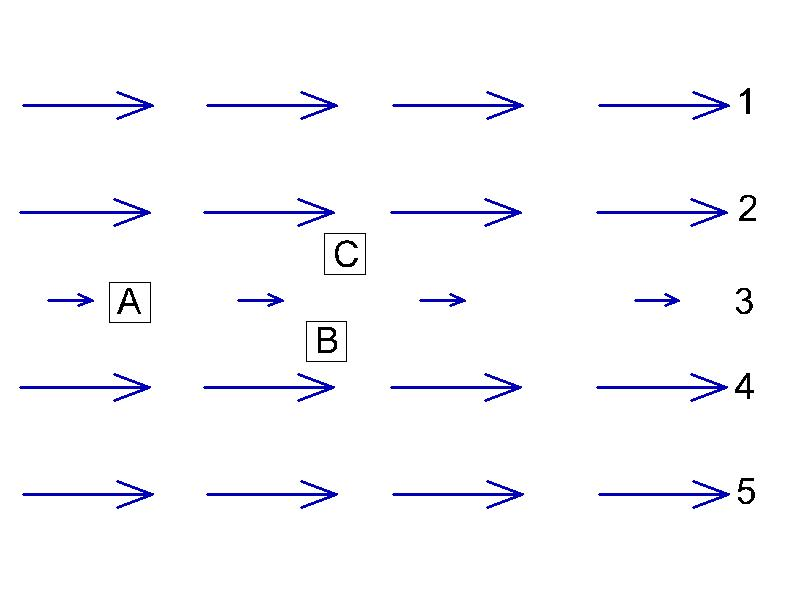
\includegraphics[width=1\linewidth]{\pathtopartone/graphics/fig171}
\caption{Horizontal Vector Field}
\end{figure}

Along the horizontal direction, the vectors are the same in magnitude and direction. Going down vertically across, the magnitude changes for 2 to 3 and 3 to 4. 1 to 2 and 4 to 5 remain the same. A small area \textbf{A} placed at the location shown, can create some kind of shear on the object depending on the strength of the vector through the top and bottom of \textbf{A}. \textbf{B} on the other hand will turn counterclockwise while \textbf{C} will turn clockwise as the force created by the arrow magnitude is more at the top for \textbf{C} compared to the bottom of \textbf{C} and more at the bottom of \textbf{B} compared to the top. Hence rotation is experienced in that region. If we however consider a field shown below. That is the field whose magnitude is changing in the \textbf{x} direction.
\begin{figure}[h]
\centering
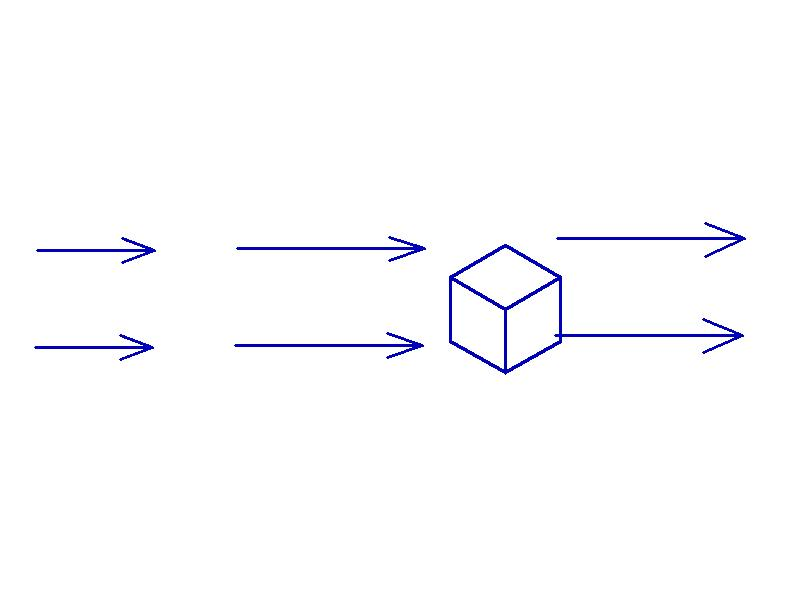
\includegraphics[width=1\linewidth]{\pathtopartone/graphics/fig172}
\caption{Changing Field Magnitude}
\end{figure}

If we put a small volume in this region and treat the field like fluid flow velocity with increasing velocity of the fluid as we move towards the right as shown by the magnitude of the arrow. The fluid coming out of the box has more value than that going into it. Hence there is a net outward flow of fluid from this volume. This kind of field will have a divergence.

Divergence is the best way to capture the effect of something either flowing out of a volume (oozing out) and the direction can be positive (net flow out of the volume) or negative (net flow into the volume).

Looking at this phenomenon where some rotation is involved, the phenomenon that can capture the effect is the \textit{curl}. Divergence and curl are the mathematical operations that capture these phenomena.

We see later when we go into electromagnetic fields, that the concept of physics is mathematically captured by the curl and divergence operators.

\subsection{Laplacian operator}
Another operator defined in terms of the del operator $\nabla$ is called the \textbf{Laplacian Operator}. It is a second-order operator denoted as $\nabla^2 = \nabla \cdot \nabla$.

If we take the $\nabla$ as a vector operator, then the dot product of the two $\nabla$ operators is given by $\nabla^2$ and it becomes a scalar operator.

\begin{dmath}
\nabla \cdot \nabla =  \left(\frac{\partial  }{\partial x}\hat x + \frac{\partial  }{\partial y}\hat y + \frac{\partial  }{\partial z}\hat z \right) \cdot \left( \frac{\partial  }{\partial x}\hat x + \frac{\partial  }{\partial y}\hat y + \frac{\partial  }{\partial z}\hat z\right)
\end{dmath}

\begin{dmath}
\frac{\partial^{2}  }{\partial x^{2}} + \frac{\partial^{2}  }{\partial y^{2}} + \frac{\partial^{2}  }{\partial z^{2}}= \nabla^{2} = \nabla \cdot \nabla
\end{dmath}

So the Laplacian operator is a second-order differential operator and the operator is a scalar operator. So to operate on a scalar quantity, it becomes $\nabla\cdot\nabla$(a scalar quantity).

For a Scalar function $f$, $\nabla^2f = \nabla \cdot (\nabla f)$ but $\nabla f =$ gradient of scalar function of $f$. The dot product in $\nabla \cdot (\nabla f) $ stands for the divergence of the gradient of $f$.

$\nabla^2 f= \nabla \cdot (\nabla f) =$ Divergence of gradient of the scalar function. The $\nabla^2 $ operator is not restricted to the scalar function only, it can operate also on vectors as $\nabla^2 \bar{F} = \nabla \cdot \nabla \bar{F}$ but this will not have meaning as we have not defined what $\nabla \bar{F}$ is.

%\begin{figure}[h]
%\centering
%\begin{minipage}{.25\textwidth}
%\centering
%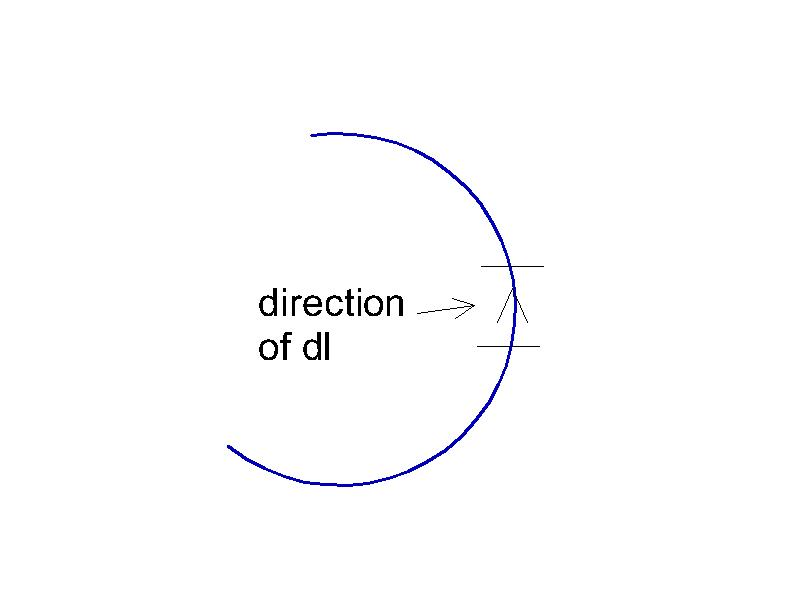
\includegraphics[width=.4\linewidth]{\pathtopartone/graphics/fig173}
%\label{fig:fig173}
%\end{minipage}%
%\begin{minipage}{.25\textwidth}
%\centering
%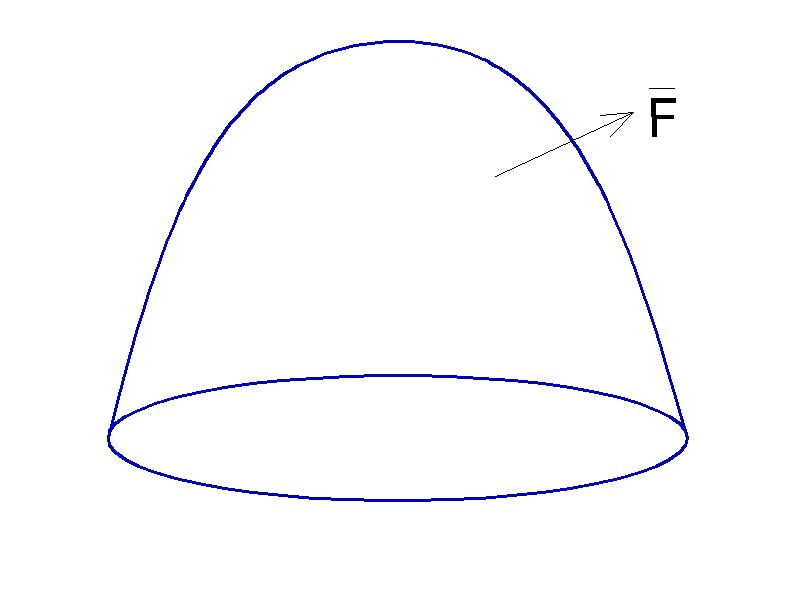
\includegraphics[width=.4\linewidth]{\pathtopartone/graphics/fig173b}
%\label{fig:fig173b}
%\end{minipage}
%\begin{minipage}{.5\textwidth}
%\centering
%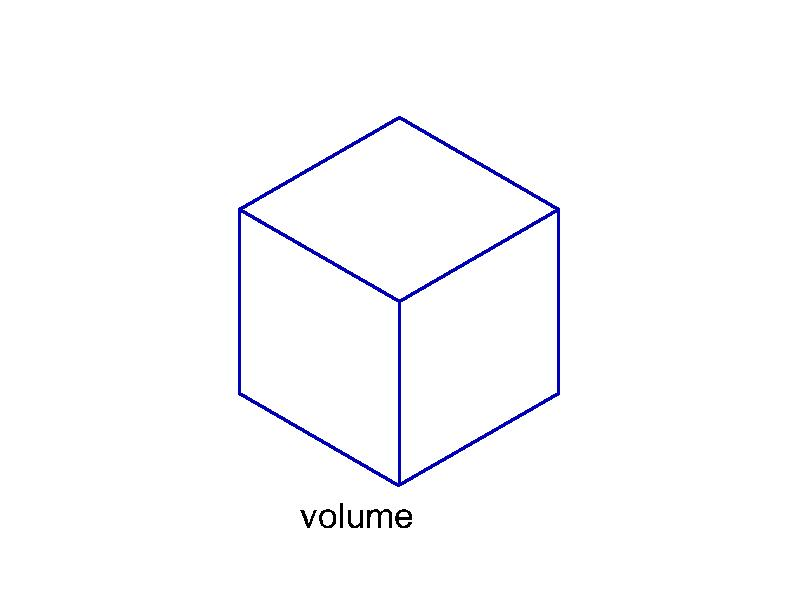
\includegraphics[width=.4\linewidth]{\pathtopartone/graphics/fig173c}
%\label{fig:fig173c}
%\end{minipage}%
%\caption{line surface and volume integration}
%\end{figure}

The DEL operator $\nabla$ can operate as either a divergence or a curl. So in this case, we take $\nabla^2$ and operate it directly on the vector quantity so that:
\begin{dmath}
\nabla^{2} \bar{F} = \frac{\partial ^ {2}}{\partial x^{2}}(\bar{F}) + \frac{\partial ^ {2}}{\partial y^{2}}(\bar{F}) + \frac{\partial ^ {2}}{\partial z^{2}}(\bar{F})
\end{dmath}
That is we take the second order differential of all the components that make up $\bar{F}$ i.e
\begin{equation*}
\bar{F} = F_{x}\hat x + F_{y}\hat y + F_{z}\hat z
\end{equation*}
So that
\begin{dmath}
\nabla^{2} \bar{F} = \frac{\partial ^ {2}}{\partial x^{2}}(F_{x}\hat x + F_{y}\hat y + F_{z}\hat z) + \frac{\partial ^ {2}}{\partial y^{2}}(F_{x}\hat x + F_{y}\hat y + F_{z}\hat z) + 
\frac{\partial ^ {2}}{\partial z^{2}}(F_{x}\hat x + F_{y}\hat y + F_{z}\hat z)
\end{dmath}
Then we combine individual components to have
\begin{dmath*}
\nabla^{2}F = (\frac{\partial ^{2} Fx}{\partial x^2} + \frac{\partial ^{2} Fx}{\partial y^2} + \frac{\partial ^{2} Fx}{\partial z^2})\hat{x} + (\frac{\partial ^{2} Fy}{\partial x^2} + \frac{\partial ^{2} Fy}{\partial y^2} + \frac{\partial ^{2} Fy}{\partial z^2})\hat{y} + (\frac{\partial ^{2} Fz}{\partial x^2} + \frac{\partial ^{2} Fz}{\partial y^2} + \frac{\partial ^{2} Fz}{\partial z^2})\hat{z}
\end{dmath*}
\begin{dmath}
\nabla^{2}F_x \hat x + \nabla^{2}F_y \hat y + \nabla^{2}F_z \hat z = \nabla^{2}\bar{F}
\end{dmath}
Later we shall see that this operation will be required when solving the problem of electro-magnetics.

\subsection{Integral Operators}

\textbf{We have been dealing with differential operators up to this point now we have to deal with integral operators which have to do with the integration of the vector fields.} If we have a vector field, there is a possibility that we can take the integral of this vector field in a plane, along the contour, or a path. It is possible that we can take the integration of this vector on a surface which can be an open or closed surface. Or we can take the integral over a volume. 

% insert image here
When we do the integration along a path, it is called \textbf{Contour or Line Integration}, while integration over a surface we call \textbf{Surface Integration}. And since a surface is two-dimensional in nature, we have a double integral.
\begin{figure}[h]
\centering
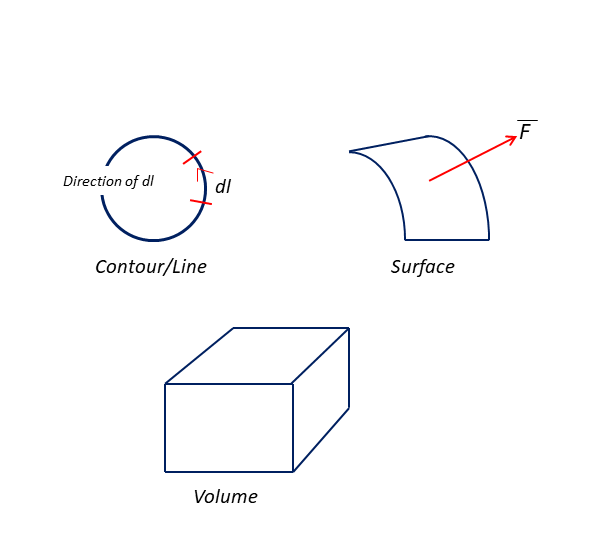
\includegraphics[width=1\linewidth]{\pathtopartone/graphics/fig17.3}
\caption{line surface and volume integration}
\end{figure}

So the contour integration is a single integration, for a volume integration, it will be a triple integration i.e. in the three-dimensional space.

We have important theorems which connect line integrals to surface integrals and surface integrals to volume integrals. We may need to change from one type of integral to another integral type e.g. from line integral to surface integral or from surface integral to volume integral.

It should be kept in mind however that integral is a Scalar quantity. Thus the final answer after integration will always be a Scalar quantity. We can define line, surface, and volume integration if we take some vector $\bar{A}$ i.e. $\bar{A}$ is a vector field. 

\subsection{Line Integral}
The line integration around some path C is ${\displaystyle \int  \bar{A} \cdot \bar{dl}}$. If we integrate along the contour in the direction shown, $dl$ has both magnitude and direction. If the path is a closed path, or mathematically we say if the contour is a closed contour, we have a closed line integral $= {\displaystyle \oint  \bar{A} \cdot \bar{dl}}$.

\begin{equation}
{\displaystyle \int  \bar{A} \cdot \bar{dl} = }open\; contour\quad while, \newline  {\displaystyle \oint  \bar{A} \cdot \bar{dl}= }closed\; contour
\end{equation}
\begin{figure}
\centering
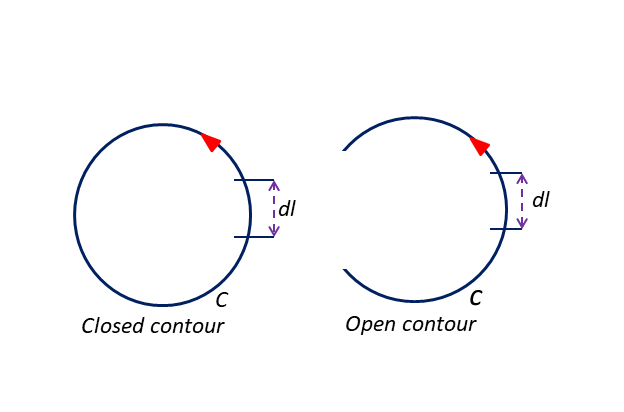
\includegraphics[width=0.9\linewidth]{\pathtopartone/graphics/fig17.4}
\caption{Open and closed contour}
\end{figure}

So at every location, we find out the product $\bar{A} \cdot \bar{dl}$ and sum it all up. This is the basis for the line integral.
\subsection{Surface Integral for Infinitesimally small Area}
We can carry out a similar operation for the surface integral as having an area $A$ with an infinitesimally small area $d\bar{A}$. $d\bar{A}$ has a direction perpendicular to that small area, if the vector field in this area is $\bar{A}$, we can define the surface integration as:
\begin{figure}
\centering
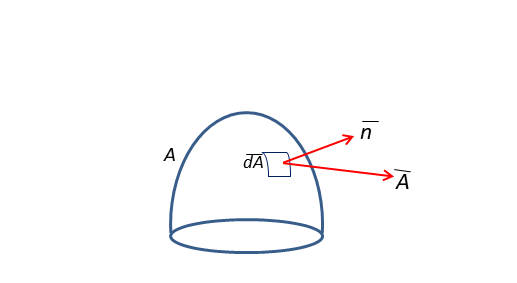
\includegraphics[width=1\linewidth]{\pathtopartone/graphics/surface_Int}
\caption{Surface Integral}
\end{figure}
%insert integration image here
(the surface may be closed or open, here it is an open surface).

Surface Integral =
\begin{equation*}
\iint \bar{A} \cdot d\bar{A}= \text{open surface}
\end{equation*}
\begin{equation}
\oiint \bar{A} \cdot d\bar{A} = \text{closed surface}
\end{equation}

$\bar{A} \cdot d\bar{A}$ is a scalar quantity so that the integration is also a scalar quantity. Now the direction for $d\bar{A}$ is thus; if it is a closed surface, the direction is taken as the outward normal for the volume created by the closed surface and it is in the positive normal direction.

If it is an Open Surface there is no preference for defining the $unit$ $normal$. We can define the $unit$ $normal$ in either direction.

$n_1$ and $n_2$ are valid unit normal for Surface \textbf{S}.

However, later on when we try to connect the contours to the surface for an open surface, then at that time we follow the convention of the right-hand rule. That is for any open surface to know the positive unit normal, just let the curl of the finger go counter-clockwise around the surface, and the direction to the thumb points in the positive direction of the unit normal to that surface.
%insert image

\subsection{Volume Integral}
The third is the volume integral, if we have some function which is a Scalar $f$:
\begin{dmath*}
\text{Volume integral} = \iiint fdV
\end{dmath*}

\begin{figure}
\centering
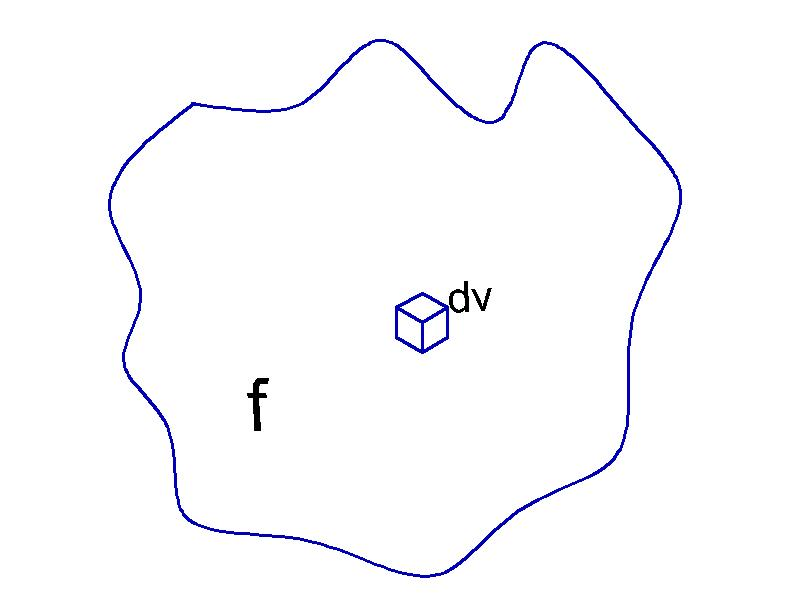
\includegraphics[width=0.7\linewidth]{\pathtopartone/graphics/fig175}
\caption{volume integral of scalar f}
\label{fig:page-8}
\end{figure}

Now when we try to relate the different integrals, ie, the line integral to the surface integral and surface integral to a volume integral, essentially the vector fields are operated on by the DEL $\nabla$ operators, then there is a relationship between these del operated fields in the integration domain. So two important theorems essentially relate this i.e. they are called the \textbf{Divergence theorem} and the \textbf{Stokes theorem}.

\subsection {Divergence Theorem}
This converts a surface integral for a vector field to a volume integral. \textbf{This converts a surface integral for a vector field to a volume integral.} If we have a vector field $\bar{A}$, then the divergence theorem states that for a \textbf{closed surface}, we have that:
\begin{equation}
\oiint \bar{A} \cdot \bar{da} = \iiint (\nabla \cdot \bar{A})dV
\end{equation}

%insert images here

So if we have a volume bounded by surface $S$, if we have a vector $\bar{A}$ and we know the surface integral of this vector i.e $\oiint \bar{A}\cdot\bar{da}$, it can be converted into a volume integral.


So $\oiint \bar{A} \cdot \bar{da} = \iiint (\nabla \cdot \bar{A})dV$ is called the divergence theorem. So when we have to convert between closed surface integral and volume integral, this theorem comes in very handy.

\subsection{Stokes Theorem}
It converts a closed line integral to an open surface integral or vice-versa.

\footnote{
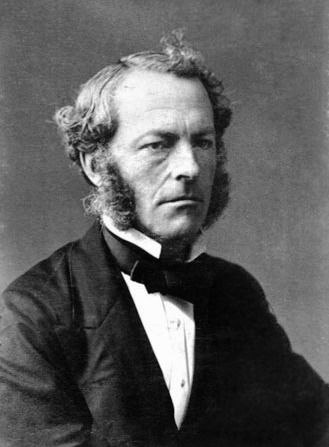
\includegraphics[scale=0.05]{\pathtopartone/graphics/georgestokes.png}
Charles George Gabriel Stokes, 1st Baronet, 1819-1903, Irish physicist and mathematician at the University of Cambridge, made contributions to the Navier-Stokes equation and to physics, optics, polarization, and fluorescence.
}

\begin{figure}[h]
\centering
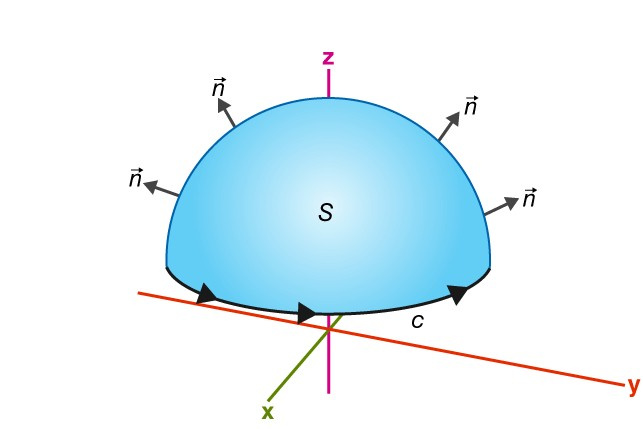
\includegraphics[width=0.7\linewidth]{\pathtopartone/graphics/fig17.8}
\caption{Stokes theorem}
\end{figure}

%\begin{figure}[h]
%\centering
%\begin{minipage}{.25\textwidth}
%\centering
%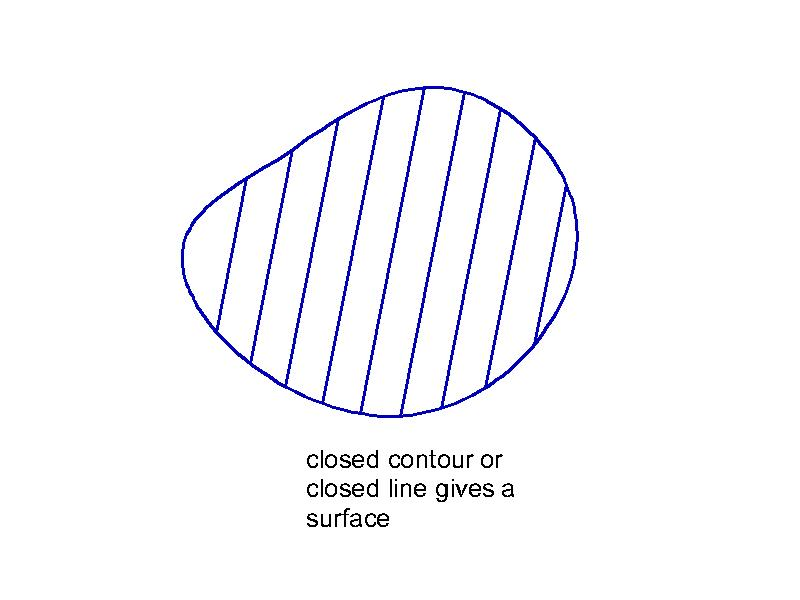
\includegraphics[width=.4\linewidth]{\pathtopartone/graphics/fig176}
%\label{fig:fig176}
%\end{minipage}%
%\begin{minipage}{.25\textwidth}
%\centering
%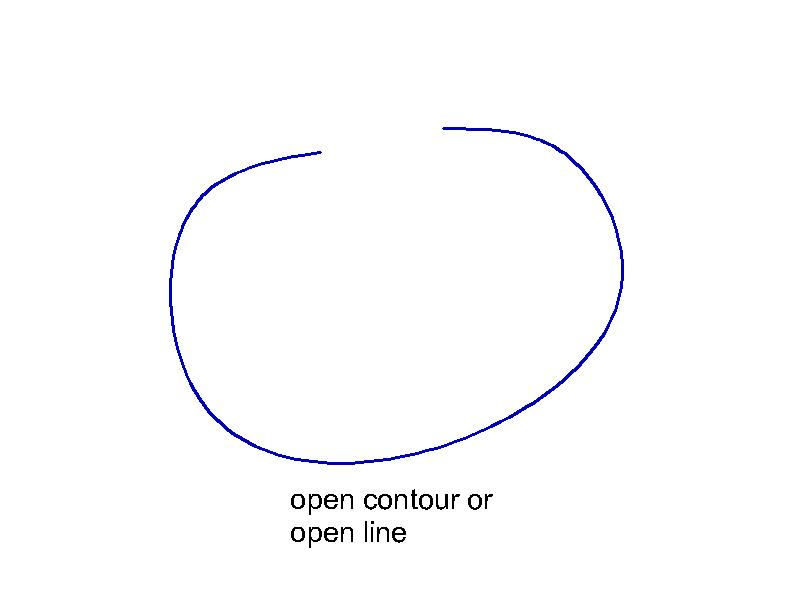
\includegraphics[width=.4\linewidth]{\pathtopartone/graphics/fig176b}
%\label{fig:fig176b}
%\end{minipage}
%\begin{minipage}{.5\textwidth}
%\centering
%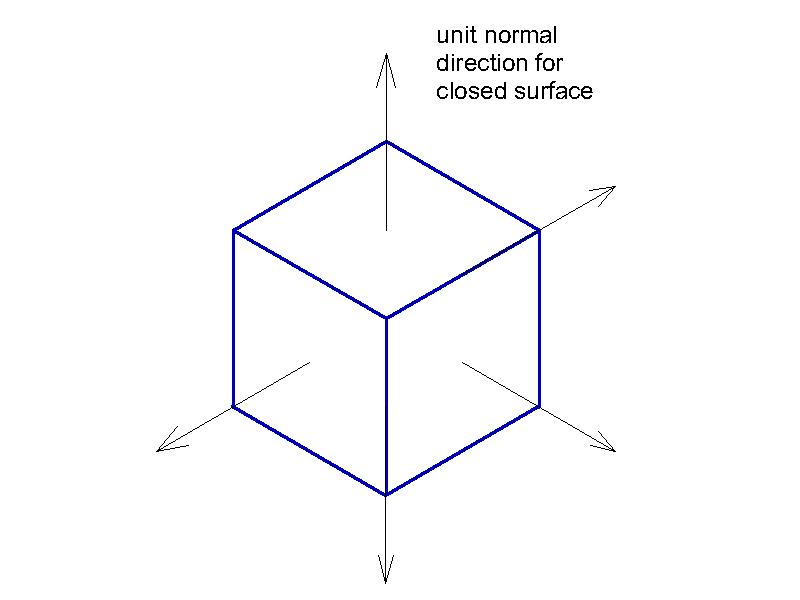
\includegraphics[width=.4\linewidth]{\pathtopartone/graphics/fig176c}
%\label{fig:fig176c}
%\end{minipage}%
%\caption{surface integral to volume integral conversion}
%\end{figure}

The surface shown is open and we have the boundary defined by contour $C$. Now we can have a small area with unit vector $\hat{n}$.

Then we can have the contour $C$ for which line integral was defined for vector $\bar{A}$. So \emph{how do we define the path $C$ with respect to $\hat{n}$?}. The convention is to follow the right-hand rule. If our contour as shown is going anticlockwise, then $\hat{n}$ goes outward, if it goes clockwise $\hat{n}$ goes inward.

%Let us illustrate this better with a very clear diagram. 
\begin{figure}
\centering
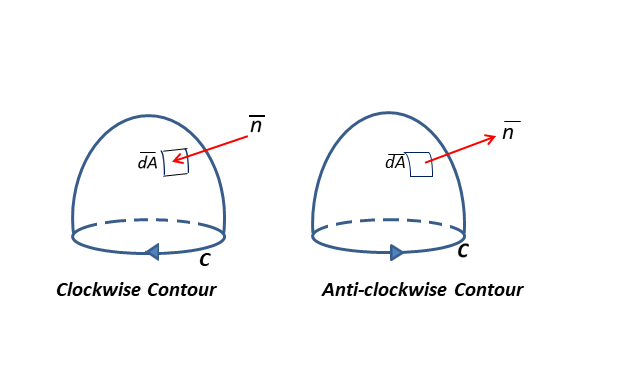
\includegraphics[width=1.2\linewidth]{\pathtopartone/graphics/contour_integral}
\caption{Contour Integration}
\end{figure}

Note that the bottom of the surface is open as compared to when this was not the case in the divergence theorem example. For these open surface $S$ bounded by closed contour $C$ the Stokes theorem states that:
\begin{equation}
\oint_c \bar{A} \cdot \bar{dl} = \iint_s  (\nabla \times \bar{A})\cdot\bar{da}
\end{equation}

So this theorem can be used to convert a line integral to a surface integral or vice-versa.

\begin{mdframed}[ backgroundcolor=lightblue, linewidth=1pt, hidealllines=true]
\subsection*{Summary}
To summarize all these again, if we have a closed surface, the closed surface integral and the integral of the volume enclosed by that closed surface can be related by the divergence theorem.
\begin{equation}
\oiint \bar{A}\cdot\bar{dA} = \iiint_v(\nabla\cdot\bar{A})dV
\end{equation}
For an open surface whose boundary at the open end is defined by a closed line path or contour, the line integral of that closed contour and the surface integral in the open surface are related by \emph{Stokes Theorem}.
\begin{equation}
\oint\bar{A}\cdot\bar{dl} = \iint_s(\nabla\times\bar{A})\cdot d\bar{a}
\end{equation}	
Later on for solving the problem of electro-magnetics, when we write \emph{Maxwell's Equation} in integral and differential forms, the two theorems become very important and handy in converting from integral to differential forms. Having understood the basics of vectors, now we can go to the basic quantities of electro-magnetics which we are going to make use of in further analysis, that is the quantities like electric and magnetic fields.

The origin of the electromagnetic phenomenon is based on the basic \emph{CHARGE}. So if we consider a charge, we know in the form of \emph{Coulombs} law that the charge has an effect all around it. If you put another charge in the vicinity of that charge, it experiences a force. This quantity is measured by an effect called the \emph{electric field}.

So if we take a charge and go in the vicinity of that charge, we experience a force that is characterized by a quantity called the electric field. However, if we put this charge in motion, then it constitutes a current as the current is nothing but the movement of charge or rate of change of charge.

So if the charge starts moving, that means you have a sustained flow of charges that gives you current, and then you have magnetic fields. So some charge when it is steady or stationary, it gives you an electric field, when it starts moving, it gives you current and that gives you a magnetic field.

The charge can accelerate also, then if we accelerate the charges, then it gives you an electric and magnetic field. So essentially we are dealing with these quantities here; the charges, current, electric, and magnetic fields and try to establish the relationship between these quantities. The relationship we have between these quantities is given by what is called \emph{Maxwell's Equations}\index{maxwell's equation}. So essentially now starting with the basics of these quantities, we would try to establish a relationship between these laws of physics in mathematical form using vector notation and vector theorems which we establish, we get Maxwell's equation. So the quantity that we have now as the first quantity is electric field $\bar{E}$ which is nothing but the force per unit charge. The electric field is a vector quantity. It has both magnitude and direction. It has V/m as its unit. Then we have a media property. Let's say we measure the electric field in a vacuum, we experience a certain force on a unit charge. If we measure the same thing and change the medium parameter to some other dielectric, then the force measured will change. So the quantity that does not depend on any parameter is the electric displacement vector $\bar{D}$.
So electric field is a quantity that is related to the charge producing the field and is also affected by the medium parameter which is called the permittivity of the medium. So we have a medium parameter called permittivity $\varepsilon$ and has unit Farad/m. If the medium parameter changes, the permittivity changes, and the electric field $\bar{E}$ measured at that point changes. Permittivity of vacuum or free space is denoted by $\varepsilon_{0} =\frac{1}{36\pi}$ $\times 10^{-9}F/m$. Sometimes written as 8.86$\times10^{-12}F/m.$
If we take another medium whose permittivity is $\varepsilon$, the ratio $\frac{\varepsilon}{\varepsilon_{0}}$ is what is called the dielectric constant for the material or relative permittivity. 
Dielectric constant $\varepsilon_{r}\equiv$ relative permittivity= $\frac{\varepsilon}{\varepsilon_{0}}$.
The quantity which is independent of the medium parameter is the displacement vector $\bar{D}=\varepsilon \bar{E}$

For a given property change, the $\bar{E}$ changes, and $\bar{D}$ remains the same, as it only depends upon the charge that is creating the field. The quantity $\varepsilon$ in a general medium can be constant everywhere or it can vary as a function of space in three-dimensional space. It can also depend on the direction, which means if we measure permittivity in the x direction, its value may vary from that in the y and z direction. So in general, the quantity  $\varepsilon$  can be direction-dependent, or it may be space-dependent. When  $\varepsilon$  varies as a function of space, we call the medium \textbf{INHOMOGENOUS MEDIUM}. If  $\varepsilon$  is direction-dependent, then the medium is called an ANISOTROPIC MEDIUM. If  $\varepsilon$ does not vary as a function of space, we call it \textbf{HOMOGENOUS MEDIUM}. If it does not vary with direction, we call that medium \textbf{ISOTROPIC MEDIUM}.
However, we will be dealing with media that are homogenous and isotropic. This means that the dielectric constant of the medium, which we shall consider, has  $\varepsilon$ that is constant in space and does not change with direction. However, if  $\varepsilon$  was anisotropic, then  $\varepsilon$  becomes a $3\times 3$ matrix of  $\varepsilon$  multiplied by vector $\bar{E}$ . For isotropic medium  $\varepsilon$  is a scalar quantity. So for this course, we deal with the medium where  $\varepsilon$  is a scalar quantity.
So in a homogeneous and isotropic medium,  $\bar{D}$ is a scalar version of  $\bar{E}$. Comparing  $\bar{D}$ and  $\bar{E}$, they have different magnitudes but with the same direction. However, if the medium were to be anisotropic,  $\varepsilon$ is a $3\times 3$ matrix and it rotates the vector  $\bar{E}$ and in general  $\bar{D}$ and  $\bar{E}$ are not in the same direction.

\begin{minipage}{1\linewidth}
\centering
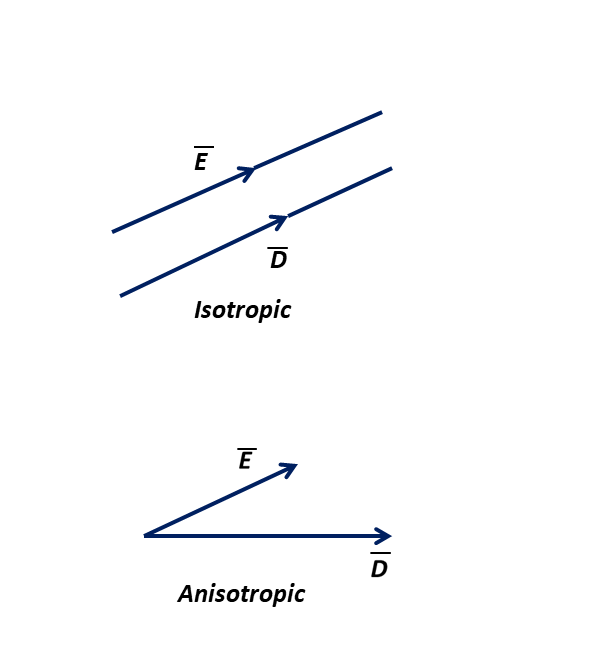
\includegraphics[width=0.7\linewidth]{\pathtopartone/graphics/isotropicAniso}
\captionof{figure}{Isotropic and Anisotropic Medium}
\label{fig:isotropicAniso}
\end{minipage}

Now we have another quantity that is very useful that we have to define, the \emph{Electric Potential} of the field. The electric field is related to the electric  potential V (scalar ) by 
$\bar{E}$= -$\nabla $ V.
So if we know the potential at a point, we can take the gradient to get the electric field at that location. From here we get the unit of the electric field. So if we find the potential, the unit of V is Volts. The del operator is a differential spatial operator$\frac{d}{dx}$ ; i.e $\frac{1}{l} or\frac{1}{m}$ that gives unit of electric field, which is V/m. So this relation of finding out the electric field from the potential comes in very handy whenever we want to find the electric field in a general complex distribution of charges. If we find the electric field  $\bar{E}$ at a particular location and find the component of the electric field for each of the charges that are distributed in space, we carry out vector additions at that point for the electric fields. It is however easier to find the potential of the different charges and add them together. The negative gradient of that gives you the electric field. So these are the basic quantities for representing the electrostatic parameters; the electric field  $\bar{E}$ and the electric potential $V$.
\end{mdframed}


\begin{mdframed}[ backgroundcolor=lightblue, linewidth=1pt, hidealllines=true]
\section{EXERCISES}
\begin{ExerciseList}
\Exercise[label={ex171}] 
How is the divergence of a vector field expressed mathematically?
\Exercise[label={ex172}] 
How is the curl of a vector field expressed mathematically?
\Exercise[label={ex173}] 
What is the Laplace operator? Also, what is its mathematical expression?
\Exercise[label={ex174}]  Integral operators have to do with the integration of the vector field. True/False
% \item Prove that $\nabla^2 \mathbf{F} = \nabla^2 F_x \mathbf{x} + \nabla^2 F_y \mathbf{y} + \nabla^2 F_z \mathbf{z}$
\Exercise[label={ex175}]
Explain the geometric interpretation of a surface integral and how it relates to the flux of a vector field through a surface.


\Exercise[label={ex176}]
State and explain the divergence theorem and its relationship to surface integrals.

% \Exercise[label={ex177}] 
% How does the divergence theorem establish a connection between a volume integral and a surface integral involving a vector field?

\Exercise[label={ex178}] 
Compare and contrast the physical interpretations of line integrals, surface integrals, and volume integrals. How do these integrals capture different aspects of a mathematical model, and in what scenarios would one choose volume integrals over the other types?


\Exercise[label={ex179}] 
What is the Divergence Theorem, and how does it establish a relationship between a volume integral and a surface integral involving a vector field?

\Exercise[label={ex1710}] 
Explain how the Divergence Theorem is used in electromagnetics, specifically in the context of electric flux and Gauss's Law.


% \Exercise[label={ex1711}] 
%  Discuss practical engineering scenarios where the Divergence Theorem is applied. How does it simplify problem-solving in fluid mechanics or heat transfer, for example?

\Exercise[label={ex1712}] 
Explain the statement and significance of Stokes' Theorem. How does it relate the circulation of a vector field around a closed curve to the behavior of the field on the surface enclosed by the curve?

Use the Divergence Theorem to find the outward flux of \( \mathbf{F} \) across the boundary of the region.

% 	\Exercise[label={ex1713}] 
% What is the electric potential energy of two electrons separated by 5.0 mm? If the separation increases, does the potential energy decrease or increase?
% \Answer
% \[ u = 2.28 \times 10^{-19} \]

% \Exercise[label={ex1714}] 
% The electric field inside a non-conducting sphere of radius $R$ with charge spread uniformly throughout its volume is radially directed and has magnitude:
% \[ E(r) = \frac{q}{4\pi\varepsilon_0 R^3} \]

% Taking $V=0$ at the center of the sphere, find the electric potential $V$ inside the sphere.
% \Exercise[label={ex1715}] 
% Calculate the average magnitude of the electric field between two points with a potential difference of 150 V between them and are separated by a distance of 2.5 cm.
% \Answer 6.0 x 10^3 v/m

% \Exercise[label={ex1716}] 
%  An electric field is expressed as $\mathbf{E} = 2\mathbf{j} + 3\mathbf{j}$. Find the potential difference ($V_A - V_B$) between two points $A$ and $B$ whose position vectors are given by $\mathbf{r}_A = \mathbf{i} + 2\mathbf{j}$ and $\mathbf{r}_B = 2\mathbf{i} + \mathbf{j} + 3\mathbf{k}$.
% \Answer V_a - V_b = -1 

% \Exercise[label={ex1717}] 
%  For an isotropic radiator, the electric field intensity at a distance $R$ is measured as $3 \, \text{V/m}$. What will be the electric field intensity at a distance $3R$?
% \Answer 1v/m.

\end{ExerciseList}
\end{mdframed}
